\documentclass[11pt,a4paper]{article}
\usepackage[T1]{fontenc}
\usepackage[utf8]{inputenc}
\usepackage{lmodern,microtype}
\usepackage{amsmath,amssymb,amsthm,mathtools}
\usepackage{booktabs,longtable,array}
\usepackage{graphicx}
\usepackage[margin=2.6cm]{geometry}
\usepackage{xcolor}
\usepackage[colorlinks=true,linkcolor=blue!50!black,citecolor=blue!50!black,urlcolor=blue!50!black]{hyperref}
\usepackage{enumitem}
\usepackage{seqsplit}
\setlist{itemsep=2pt,topsep=4pt}
\emergencystretch=3em

\newtheorem{theorem}{Theorem}[section]
\newtheorem{proposition}[theorem]{Proposition}
\newtheorem{lemma}[theorem]{Lemma}
\newtheorem{corollary}[theorem]{Corollary}
\theoremstyle{definition}
\newtheorem{definition}[theorem]{Definition}
\newtheorem{remark}[theorem]{Remark}
\newtheorem{example}[theorem]{Example}

\newcommand{\N}{\mathbb{N}}
\newcommand{\Z}{\mathbb{Z}}
\newcommand{\nest}{\mathbin{\perp}}
\newcommand{\Sig}{\Sigma}
\newcommand{\Ret}{\mathcal{R}}
\DeclareMathOperator{\vp}{v}
\newcommand{\Wa}{W_{45}}
\newcommand{\Wb}{W_{11}}

\title{Autonomous Aperiodicity in the UNNS Substrate:\\ An Expanding Arithmetic Return Theorem}
\author{UNNS Research Collective}
\date{Version 2.7 \,--\, November 2026}

\begin{document}
\maketitle

\begin{abstract}
\noindent
The UNNS Substrate generates integers by the nest operation $M\nest N=M(N+1)^2/N$, whose integer values occur exactly on the anchors $N\mid M$. If the current integer selects, from a fixed finite list of nests, the first one that anchors it, the result is an autonomous, stationary arithmetic dynamics with no external input. We study the four-prime instance: the $22$ nests $N\ge 2$ for which $N$ and $N+1$ are both $\{2,3,5,7\}$-smooth, a fixed priority order, and the seed $x_0=2^4 3^6 5^4 7^3$. On the section $\Sigma=\{5^z,\,2\cdot5^z: z\ge 50000\}$ we prove an \emph{expanding return theorem}: the selected return (the first later state in $\Sigma$ with $z'\ge 10z$) exists for every state and is given exactly by $z'=(2869\,z+\delta_{a,r})/49$, $r=z\bmod 49$, with $\delta_{a,r}\in[-7737,\,27275]$ from an explicit table; the branch $a=1$ reduces to $a=0$ by a seven-move lemma, $\Ret(2\cdot5^z)=\Ret(5^{z+8})$. The orbit from $x_0$, which enters $\Sigma$ at step $1{,}039{,}587$, therefore has a selection itinerary that is not eventually periodic. We explain the structure: every round consists of three regimes governed by the grammar---a rotation on $\mathbb{Z}/9\times\mathbb{Z}/5$ among the top three moves (period $45$), a register cycle of period $11$, and a single-move run---which transfer the exponent of $5$ into that of $7$, then $2$, then $5$ again, at the exact exchange rates $49\!:\!151$, $2\!:\!38$, $2\!:\!2$ of the three block vectors; their product is the gain $2869/49$. The finite bounded transients between regimes, which fix the correction table, are certified by a computer-assisted proof ($196$ symbolic families, $99{,}866$ exact obligations, one independent re-implementation).
\end{abstract}

\paragraph{Keywords.} UNNS Substrate; nest operation; autonomous selection; arithmetic dynamics; return map; exchange cycle; non-periodicity; computer-assisted proof.

%% ------------------------------------------------------------------
\section{Introduction}\label{sec:intro}

The UNNS Substrate begins from a single arithmetic act: an integer $N$ serves as a \emph{nest} around which values are generated, and the generated value at position $M$ is $M\nest N = MN + M/N + 2M$. Most positions give fractions; the integer values, the \emph{anchors}, occur exactly when $N\mid M$, and then $M\nest N = k(N+1)^2$ for $M=kN$ (the Integer Ray Theorem of the UNNS introduction \cite{unns-intro}). The arithmetic transition $x\mapsto x(N+1)^2/N$ with $N\mid x$, the graph it generates, and the prime-valuation reduction of its moves are developed in the source releases of the UNNS arithmetic-dynamics collection \cite{ad-collection,u4gen,u2001}. The programme asks which generated structures are merely produced, which lie on distinguished routes, and which can be generated at all under a stated rule.

This paper studies the simplest way in which such a generative rule can run \emph{by itself}. Take a finite list of nests, ordered by priority. At each stage the current integer is anchored by some of them; let the first anchoring nest in the list act. The result is a deterministic dynamics on the integers in which nothing is supplied from outside: the state selects its own next generative act. The sequence of selected nests is the \emph{selection itinerary}.

\paragraph{Question.} Can such an autonomous selector produce a selection itinerary that is provably \emph{not} eventually periodic, with the proof resting on an exact structural law rather than on long numerical trajectories, and can that law be traced back to the arithmetic of the nests?

\paragraph{Answer for one explicit instance.} We answer affirmatively for the four-prime construction (\S\ref{sec:construction}): the $22$ admissible nests over $\{2,3,5,7\}$, one fixed priority order, one seed. Our results are:
\begin{enumerate}[label=(\arabic*)]
\item \textbf{The grammar and its autonomous selector} (\S\ref{sec:grammar}--\ref{sec:selection}): anchor arrows $m\to m\nest N$, their exponent-translation law, strict growth and acyclicity, and the stationary priority selector.
\item \textbf{The exact four-prime construction} (\S\ref{sec:construction}).
\item \textbf{The expanding return theorem} (Theorem~\ref{thm:return}): on $\Sig$ the selected return is $z'=(2869z+\delta_{a,r})/49$, with an explicit table, $z'\ge10z$, and the reduction $\Ret(2\cdot5^z)=\Ret(5^{z+8})$ (Proposition~\ref{prop:reduction}).
\item \textbf{A mechanism} (\S\ref{sec:mechanism}): the round splits into three regimes, each a small exactly solvable system---a rotation on $\mathbb{Z}/9\times\mathbb{Z}/5$, a register cycle, a single-move run---that move the exponent of $5$ to $7$ to $2$ and back to $5$ at fixed exchange rates. This derives the gain $2869/49$, the block slopes $2,151,2869$, the modulus $98$, the parity rule for $a'$, and the congruence $\delta\equiv-27r\pmod{49}$, from the grammar rather than from the certificate.
\item \textbf{Non-eventually-periodic itinerary} (Theorem~\ref{thm:aper}).
\item \textbf{Proof, independent verification, mathematical significance, and consequences} (\S\ref{sec:proof}--\ref{sec:signif}).
\end{enumerate}

\paragraph{Scope.} The orbit is strictly increasing and therefore trivially non-periodic (Proposition~\ref{prop:trivial}); the substantive statement concerns the \emph{itinerary}. The paper establishes the exact return law of the selector on the section $\Sig$, derives it from a three-regime exchange mechanism of the grammar, and certifies the finite corrections by a computer-assisted proof with exact integer certificates and an independent re-implementation. The result concerns the selector for one priority list, one prime set and one seed.

%% ------------------------------------------------------------------
\section{The UNNS arithmetic transition grammar}\label{sec:grammar}

\begin{definition}[Nest operation and anchor]\label{def:nest}
For integers $M\ge1$ and $N\ge1$ let $M\nest N := MN + M/N + 2M = M(N+1)^2/N$. We say that $M$ is an \emph{anchor of the nest $N$} if $M\nest N\in\Z$.
\end{definition}

\begin{lemma}[Anchors, \cite{unns-intro}]\label{lem:anchor}
$M$ is an anchor of $N$ if and only if $N\mid M$; in that case $M=kN$ and $M\nest N = k(N+1)^2$.
\end{lemma}
\begin{proof}
$M(N+1)^2/N\in\Z$ iff $N\mid M(N+1)^2$, and $\gcd(N,N+1)=1$ gives $\gcd(N,(N+1)^2)=1$. The value is then $(M/N)(N+1)^2$.
\end{proof}

\begin{definition}[Anchor arrow]\label{def:arrow}
For $N\ge 2$ and $m\in\N$ with $N\mid m$ write $m\xrightarrow{N} m':=m\nest N$. Equivalently, if $m=Nq$ then $m'=(N+1)^2q$: the factor $N$ is \emph{substituted} by the square of its successor. The set of \emph{admissible arrows at $m$} is $\{N\ge2: N\mid m\}$.
\end{definition}

\begin{remark}\label{rem:unit}
The unit nest $N=1$ generates the universally admissible transition $m\mapsto 4m$. We restrict the autonomous transition grammar to proper nests $N\ge 2$, so that move admissibility is governed by nontrivial divisibility conditions. This is a convention defining the system investigated here, not a restriction imposed by the underlying nest operation.
\end{remark}

\begin{remark}[Why the convention matters]\label{rem:unit2}
Since $N=1$ is admissible at every state, placing it first in a priority list would make the itinerary constant, and placing it last would make it an unconditional fallback, so that no state could ever be without an admissible move. Either way the divisibility structure studied here would be bypassed. The convention also accounts for the count in Lemma~\ref{lem:moves}: the pair $(1,2)$ of consecutive smooth integers gives the excluded nest $N=1$, leaving $22$ of the $23$ Størmer pairs.
\end{remark}

\begin{lemma}[Exponent translation, growth, acyclicity]\label{lem:exp}
Let $N\ge 2$ and $m\xrightarrow{N}m'$. Then:
\begin{enumerate}[label=(\roman*)]
\item for every prime $p$, $\vp_p(m') = \vp_p(m) + \Delta_p(N)$ with $\Delta_p(N):=2\vp_p(N+1)-\vp_p(N)$;
\item the arrow is admissible at $m$ iff $\vp_p(m)\ge \vp_p(N)$ for all primes $p$;
\item $m'/m = (N+1)^2/N = N+2+1/N\ge 9/2$;
\item consequently any chain of anchor arrows is strictly increasing; in particular no chain returns to a previous integer.
\end{enumerate}
\end{lemma}
\begin{proof}
(i)--(ii) are the definitions of $\vp_p$ applied to $m'=m(N+1)^2/N$ and to $N\mid m$. (iii) is direct, with minimum $9/2$ at $N=2$. (iv) follows from (iii).
\end{proof}

Lemma~\ref{lem:exp}(i)--(ii) make the grammar a system of \emph{threshold-and-translate rules on exponent vectors}: an arrow is enabled by a lower bound on the exponents and acts by adding a fixed vector. Everything below, including the mechanism of \S\ref{sec:mechanism}, is done in this form.

%% ------------------------------------------------------------------
\section{Autonomous selection}\label{sec:selection}

\begin{definition}[Stationary priority selector]\label{def:selector}
Let $L=(N_1,\dots,N_n)$ be a list of distinct integers $\ge2$. For $m\in\N$ define $\sigma_L(m):=N_i$ where $i$ is the least index with $N_i\mid m$, and $\sigma_L(m)$ undefined if there is none. The \emph{orbit} of $x_0$ is $x_{k+1}=x_k\nest\sigma_L(x_k)$, and the \emph{selection itinerary} is $\iota_k=\sigma_L(x_k)$, $k\ge0$.
\end{definition}

The selector is \emph{autonomous} (no input other than the current integer), \emph{stationary} (the rule does not depend on $k$) and \emph{local} (it depends only on which nests anchor the current integer). The only freedom is the list $L$ and the seed.

\begin{proposition}\label{prop:trivial}
If $\sigma_L(x_k)$ is defined for all $k$, the orbit $(x_k)$ is strictly increasing, hence not eventually periodic. The same does \emph{not} follow for the itinerary $(\iota_k)$, which is the object of Theorem~\ref{thm:aper}.
\end{proposition}
\begin{proof}
Lemma~\ref{lem:exp}(iii).
\end{proof}

%% ------------------------------------------------------------------
\section{The four-prime construction}\label{sec:construction}

Let $P=\{2,3,5,7\}$ and call an integer $P$-smooth if all its prime factors lie in $P$.

\begin{definition}[Move set]\label{def:moves}
$\mathcal{M}_P=\{N\ge 2:\ N \text{ and } N+1 \text{ are both } P\text{-smooth}\}$.
\end{definition}

\begin{lemma}\label{lem:moves}
$\mathcal{M}_P$ has exactly $22$ elements, the largest being $4374$ (with $4375=5^4\cdot7$). They are listed in Table~\ref{tab:moves}. If $x$ is $P$-smooth and $N\in\mathcal{M}_P$ anchors $x$, then $x\nest N$ is $P$-smooth.
\end{lemma}
\begin{proof}
By Størmer's theorem \cite{stormer} there are finitely many pairs of consecutive $P$-smooth integers, and Lehmer's method \cite{lehmer} finds them all; for the first four primes there are $23$ such pairs including $(1,2)$, the largest being $(4374,4375)$ \cite{oeis}, which gives $22$ with $N\ge2$. We also re-derived the list by exhaustive search for $N\le10^7$. The last statement holds because $x\nest N=(x/N)(N+1)^2$ and $N+1$ is $P$-smooth.
\end{proof}

\begin{definition}[The four-prime autonomous system]\label{def:system}
The list $L_4$ is the $22$ moves of Table~\ref{tab:moves} in the order shown (priority $1$ first), the seed is $x_0=2^4\,3^6\,5^4\,7^3=2{,}500{,}470{,}000$, and the system is the orbit and itinerary of Definition~\ref{def:selector} for $(L_4,x_0)$.
\end{definition}

The priority order and the seed are data of the construction, fixed in the frozen release \cite{adj4-frozen} (designated ADJ4 in the project's releases); the results below are specific to them, and we do not claim that this order is canonical.

\paragraph{Coordinates.} Every state is $P$-smooth, so $x=2^{v_2}3^{v_3}5^{v_5}7^{v_7}$ is recorded by $v=(v_2,v_3,v_5,v_7)\in\N^4$, and each move acts by $v\mapsto v+\Delta(N)$ when $v\ge \vp(N)$ componentwise (Lemma~\ref{lem:exp}). The vectors $\Delta(N)$ are in Table~\ref{tab:moves}. Four moves matter below:
\[
\begin{gathered}
\Delta(2400)=(-5,-1,-2,+8),\quad \Delta(3)=(+4,-1,0,0),\\
\Delta(35)=(+4,+4,-1,-1),\quad \Delta(4)=(-2,0,+2,0).
\end{gathered}
\]

\begin{definition}[Section and selected return]\label{def:section}
Let $\Sig=\{(a,0,z,0): a\in\{0,1\},\ z\ge 50000\}$, i.e.\ the integers $2^a5^z$. For $s\in\Sig$ the \emph{selected return} $\Ret(s)$ is the first state \emph{after} $s$ on the orbit of $s$ (under the selector) that lies in $\Sig$ and satisfies $z'\ge10z$, whenever it exists.
\end{definition}

\begin{remark}[Selected return versus first return]\label{rem:first}
$\Ret$ is not the first-return map to $\Sig$. For $a=1$ the first return to $\Sig$ occurs after seven moves, at $z+8<10z$, and is deliberately skipped (Proposition~\ref{prop:reduction}). The theorem below concerns the selected return only; no first-return statement beyond that proposition is made.
\end{remark}

%% ------------------------------------------------------------------
\section{Main results}\label{sec:results}

\begin{theorem}[Expanding arithmetic return]\label{thm:return}
For every $a\in\{0,1\}$ and every integer $z\ge50000$, the selected return of $s=2^a5^z$ exists, and equals $2^{a'}5^{z'}$ with
\begin{equation}\label{eq:return}
z'=\frac{2869\,z+\delta_{a,r}}{49},\qquad r=z \bmod 49,
\end{equation}
where $(a',\delta_{a,r})$ depends only on $(a,r)$ and is given in Table~\ref{tab:returnmap}. Moreover $a'\in\{0,1\}$, $-7737\le\delta_{a,r}\le27275$ (both bounds attained), $z'$ is an integer, and $z'\ge10z$. In particular $\Ret:\Sig\to\Sig$ is a total self-map and
\[
z'\ \ge\ 10z,\qquad \lim_{z\to\infty} z'/z=2869/49\approx 58.551.
\]
\end{theorem}

\begin{proposition}[Reduction of the branch $a=1$]\label{prop:reduction}
For every $z\ge0$ the orbit of $2\cdot5^z$ has the itinerary $(2,3,3,4,4,4,4)$ in its first seven steps and reaches $5^{z+8}$; no earlier state of these seven is of the form $2^a5^{z''}$. Consequently, for $z\ge50000$, the selected return of $(1,z)$ is that of $(0,z+8)$, and in the table of Theorem~\ref{thm:return}
\[
a'_{1,r}=a'_{0,\,r+8},\qquad \delta_{1,r}=\delta_{0,\,r+8}+22{,}952\qquad(r+8\ \text{taken mod }49).
\]
\end{proposition}
\begin{proof}
The seven states are
$(1,0,z,0)\xrightarrow{2}(0,2,z,0)\xrightarrow{3}(4,1,z,0)\xrightarrow{3}(8,0,z,0)\xrightarrow{4}(6,0,z{+}2,0)\xrightarrow{4}(4,0,z{+}4,0)\xrightarrow{4}(2,0,z{+}6,0)\xrightarrow{4}(0,0,z{+}8,0)$.
At each state the selected move is the first enabled in $L_4$: at $(1,0,z,0)$ the moves $2400,3,35,15,27$ need $v_3\ge1$ or $v_7\ge1$, $4$ needs $v_2\ge2$, $14$ needs $v_7\ge1$, and $2$ is enabled; at $(0,2,z,0)$ and $(4,1,z,0)$ the move $3$ is enabled and $2400$ is not ($v_2<5$); at $(8,0,z,0)$ and the three following states $v_3=v_7=0$, which disables $2400,3,35,15,27$, and $4$ is enabled ($v_2\ge2$). No threshold on $v_5$ is involved, so the statement holds for every $z$. The intermediate states have $v_2\ge2$ or $v_3\ne0$ and so are not of the form $2^a5^{z''}$. Since the orbit of $(1,z)$ continues as the orbit of $(0,z+8)$, its selected return is a later state on that orbit; the comparison of the two halves of Table~\ref{tab:returnmap}, $\delta_{1,r}-\delta_{0,r+8}=22{,}952=8\cdot2869$ for all $49$ residues (a finite check, \texttt{reduction\_check.py}), shows that the formula~\eqref{eq:return} for $(1,z)$ coincides with that for $(0,z+8)$.
\end{proof}

\begin{corollary}[Global description of the orbit]\label{cor:orbit}
The orbit of $x_0$ enters $\Sig$ for the first time at step $n_0=1{,}039{,}587$, at the state $(a,z)=(1,\,1{,}269{,}113)$. Writing $s_0$ for that state and $s_{j+1}=\Ret(s_j)$, the orbit visits every $s_j$, $j\ge0$, in order, and $z_{j+1}\ge10z_j$. The round from $s_j=(a,50000+\rho+98t)$ has exactly $L_0(a,\rho)+4620\,t$ moves, with $L_0(a,\rho)$ listed in the supplement. The first values are in Table~\ref{tab:returns}: $s_1$ and $s_2$ were reached by direct execution of the selector ($60{,}869{,}526$ and $3{,}563{,}973{,}091$ steps, the skipped first return $(0,1{,}269{,}121)$ occurring at step $1{,}039{,}594$); the rows $j\ge3$ are consequences of Theorem~\ref{thm:return}, not executions.
\end{corollary}

\begin{table}[h]
\centering\small
\begin{tabular}{@{}rrrrl@{}}
\toprule
$j$ & $a_j$ & $z_j$ & step $n_j$ & status\\
\midrule
0 & 1 & 1\,269\,113 & 1\,039\,587 & executed\\
1 & 0 & 74\,308\,258 & 60\,869\,526 & executed\\
2 & 0 & 4\,350\,824\,298 & 3\,563\,973\,091 & executed\\
3 & 0 & 254\,745\,202\,239 & 208\,674\,261\,405 & from Thm.~\ref{thm:return}\\
4 & 0 & 14\,915\,591\,535\,054 & 12\,218\,090\,938\,286 & from Thm.~\ref{thm:return}\\
5 & 1 & 873\,323\,104\,368\,641 & 715\,381\,691\,876\,438 & from Thm.~\ref{thm:return}\\
6 & 1 & 51\,133\,958\,906\,809\,224 & 41\,886\,328\,040\,684\,151 & from Thm.~\ref{thm:return}\\
\bottomrule
\end{tabular}
\caption{The first selected returns $s_j=2^{a_j}5^{z_j}$ and the step $n_j$ at which the orbit of $x_0$ is at $s_j$. Rows $j\ge3$ iterate the table of Theorem~\ref{thm:return} and the step law $n_{j+1}=n_j+L_0+4620t_j$.}
\label{tab:returns}
\end{table}

\begin{example}
For $s_0=(1,\,1269113)$: $r=13$, $\delta_{1,13}=19445$, so $z'=(2869\cdot1269113+19445)/49=74{,}308{,}258$, with $a'=0$. By Proposition~\ref{prop:reduction} this is the return of $(0,1269121)$, with $r=21$ and $\delta_{0,21}=-3507$: $(2869\cdot1269121-3507)/49$ gives the same value. For $s_1=(0,\,74308258)$: $r=3$, $\delta_{0,3}=-1600$, so $z'=4{,}350{,}824{,}298$. Both agree with step-by-step execution (\S\ref{sec:audit}).
\end{example}

\begin{figure}[t]
\centering
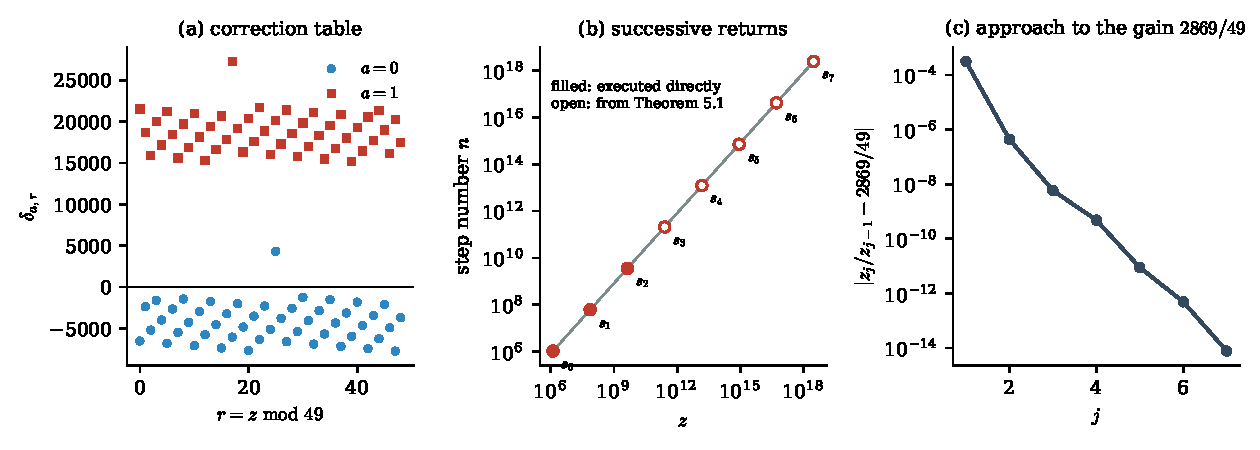
\includegraphics[width=\textwidth]{../figures/fig_returnmap2.pdf}
\caption{The return map. (a) The correction values $\delta_{a,r}$, $r=0,\dots,48$; the two outliers $\delta_{0,25}=4323$ and $\delta_{1,17}=27275$ are the entries with residual $e_1=24$ (\S\ref{subsec:balance}). (b) Step number against $z$ at $s_0,\dots,s_7$ (logarithmic axes); filled markers were executed directly, open markers follow from Theorem~\ref{thm:return}. (c) The deviation of $z_j/z_{j-1}$ from $2869/49$ decays geometrically.}
\label{fig:returnmap}
\end{figure}

\begin{theorem}[Non-eventually-periodic selection itinerary]\label{thm:aper}
The selection itinerary $(\iota_k)_{k\ge0}$ of the four-prime system $(L_4,x_0)$ is not eventually periodic. More precisely, every round $s_j\to s_{j+1}$ ends with a run of $N=4$ of length at least $2869\,t_j$, where $t_j=\lfloor (z_j-50000)/98\rfloor$, and the first move of every round is $N=2$ or $N=5$.
\end{theorem}

Theorem~\ref{thm:aper} is proved in \S\ref{sec:aper} from facts certified in \S\ref{sec:proof}; \S\ref{sec:mechanism} explains where its ingredients come from.

\begin{figure}[t]
\centering
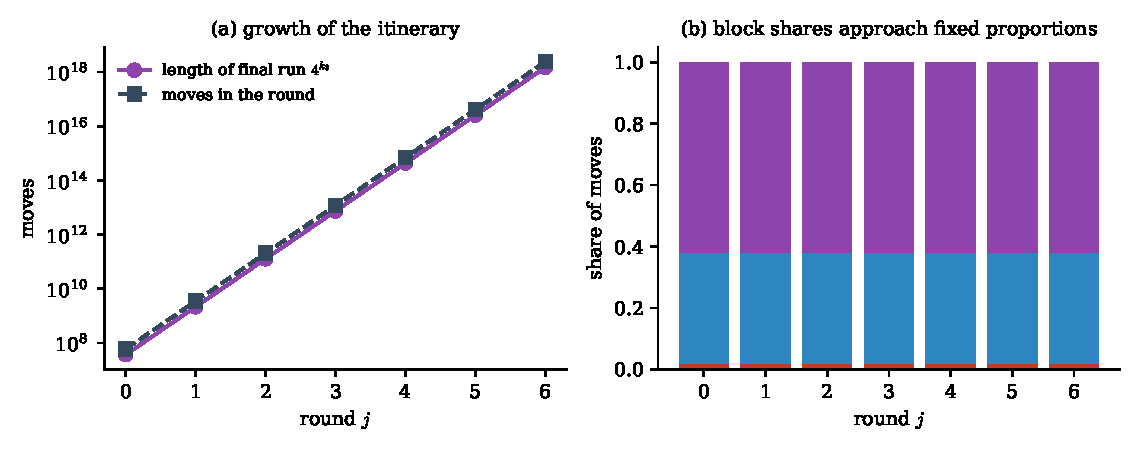
\includegraphics[width=\textwidth]{../figures/fig_itinerary.pdf}
\caption{The itinerary over successive rounds, from the iterated return map (a consequence of Theorem~\ref{thm:return}, not an execution beyond $j=2$). (a) The final run $4^{k_3}$ and the whole round grow geometrically, by the factor $2869/49$ per round. (b) The shares of the three regimes converge to approximately $1.9\%$, $36.0\%$ and $62.1\%$: since the block counts are affine in $t$ with family-dependent intercepts, the proportions are asymptotically constant, not exactly equal from round to round. The itinerary is asymptotically self-similar under $\Ret$.}
\label{fig:itinerary}
\end{figure}

%% ------------------------------------------------------------------
\section{Mechanism: three regimes and an exchange cycle}\label{sec:mechanism}

The certificate of \S\ref{sec:proof} shows that every round has the same form: bounded transients and three growing blocks. This section shows where that form comes from. Statements here are proved by hand from the exponent form of the grammar, except where a small finite enumeration is named; the enumerations are in the supplement (\texttt{register\_cycles.py}, \texttt{mechanism\_check.py}). The bounded transients between regimes are not derived here: they are what the certificate computes (\S\ref{subsec:limits-mech}).

\medskip
\noindent\textbf{Idea.} Write the state as four counters $(v_2,v_3,v_5,v_7)$. In each regime the selector uses only a few moves; some coordinates cycle within a bounded window (\emph{registers}) while others drift linearly (\emph{counters}). The drift per period is the net vector of the period; the rounds are driven by three such drifts in sequence, $5\to7\to2\to5$ (Figure~\ref{fig:exchange}).

\begin{figure}[t]
\centering
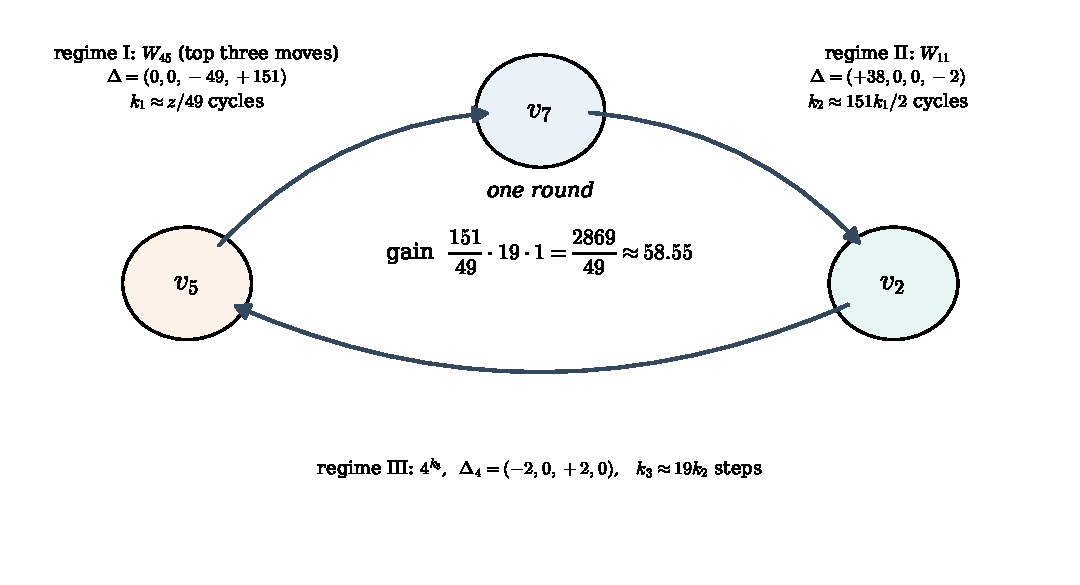
\includegraphics[width=0.9\textwidth]{../figures/fig_exchange.pdf}
\caption{The exchange cycle of one round. Regime I (the three highest-priority moves) converts exponent of $5$ into exponent of $7$, regime II converts $7$ into $2$, regime III converts $2$ back into $5$. The net vectors of the three periods fix the exchange rates and hence the gain $2869/49$ (Proposition~\ref{prop:exchange}).}
\label{fig:exchange}
\end{figure}

\subsection{Regime I: the top three moves and a rotation on \texorpdfstring{$\mathbb{Z}/9\times\mathbb{Z}/5$}{Z/9 x Z/5}}

The three highest-priority moves $2400,3,35$ have the vectors displayed in \S\ref{sec:construction}.

\begin{lemma}[A common translation]\label{lem:shift}
Each of $2400,3,35$ translates $(v_2\bmod 9,\ v_3\bmod 5)$ by the same amount $(4,4)$.
\end{lemma}
\begin{proof}
$\Delta_2\in\{-5,+4,+4\}\equiv4\pmod 9$ and $\Delta_3\in\{-1,-1,+4\}\equiv4\pmod5$.
\end{proof}

\begin{proposition}[Regime I]\label{prop:reg1}
Consider a stretch of the orbit on which the selected move always lies in $\{2400,3,35\}$ and, before each step, $v_5\ge2$ and (before each $35$) $v_7\ge1$ (``reservoir condition''). Then:
\begin{enumerate}[label=(\roman*)]
\item the selected move is $2400$ if $v_3\ge1$ and $v_2\ge5$; $3$ if $v_3\ge1$ and $v_2<5$; $35$ if $v_3=0$; so $(v_2,v_3)$ evolves autonomously by
$F(v_2,v_3)=(v_2-5,v_3-1),\ (v_2+4,v_3-1),\ (v_2+4,4)$ respectively;
\item after a finite transient, the itinerary is periodic with period $45$: it is a rotation of the word $\Wa$ displayed in \S\ref{subsec:results-cert}, which contains $20$ moves $2400$, $16$ moves $3$ and $9$ moves $35$, is primitive, and has net vector $\Delta(\Wa)=(0,0,-49,+151)$;
\item the $45$ states of the period are the $45$ points of $\mathbb{Z}/9\times\mathbb{Z}/5$, each visited once (Figure~\ref{fig:registers}a).
\end{enumerate}
\end{proposition}
\begin{proof}
(i) Since $2400,3,35$ are the first three entries of $L_4$, the selector chooses the first of them that is enabled. Under the reservoir condition $2400$ is enabled iff $v_3\ge1,v_2\ge5$; $3$ iff $v_3\ge1$; $35$ iff $v_5\ge1,v_7\ge1$, which holds; hence the rule.

(ii) The coordinate $v_3$ decreases by $1$ at each step except at $35$, which occurs only when $v_3=0$ and sets $v_3=4$. After the first $35$ the coordinate $v_3$ therefore runs $4,3,2,1,0,4,\dots$ with period $5$, and the itinerary has the form of blocks $(x_1x_2x_3x_4\,35)$, $x_i\in\{2400,3\}$. Let $u$ be $v_2$ right after a $35$ and put $s(w)=w-5$ for $w\ge5$, $s(w)=w+4$ for $w<5$, so that $x_i=2400$ iff the current $v_2\ge5$ and $v_2\mapsto s(v_2)$ along $x_1,\dots,x_4$; $35$ adds $4$. The next value is $u'=s^4(u)+4$. Since $s(w)\le\max(w-5,8)$ and $s\ge0$, we get $4\le u'\le\max(u-16,12)$: after finitely many blocks $u\in[4,12]$, and this window is then invariant. Now $s(w)\equiv w-5\pmod 9$ always, so $u'\equiv u-20+4=u-16\equiv u+2\pmod9$. Nine consecutive integers form a complete residue system modulo $9$, hence $u$ is determined by its residue and runs through the $9$ values of the window with period exactly $9$ (as $\gcd(2,9)=1$). The itinerary is thus periodic with $9$ blocks of $5$ moves, i.e.\ period $45$. Explicitly, the block for $u$ is generated by the recursion above and the nine blocks for $u=12,5,\dots$ are pairwise distinct (checked in \texttt{register\_cycles.py}), so no shorter period exists; this is the word $\Wa$, and the closed form reproduces the word printed in \S\ref{subsec:results-cert} exactly. Counting over one period with $a$ moves $2400$ and $b$ moves $3$: $a+b=36$ and $-5a+4b+4\cdot9=0$ (return of $v_2$), so $a=20$, $b=16$; then $\Delta_5=-2\cdot20-9=-49$, $\Delta_7=8\cdot20-9=151$, and $\Delta_2=\Delta_3=0$.

(iii) By Lemma~\ref{lem:shift} each step translates $(v_2\bmod9,v_3\bmod5)$ by $(4,4)$, an element of order $\operatorname{lcm}(9,5)=45$ in $\mathbb{Z}/9\times\mathbb{Z}/5$, so $45$ consecutive steps visit $45$ distinct residue pairs.
\end{proof}

\noindent The period $45=9\cdot5$ is thus not a feature of a particular orbit but of the vectors $\Delta(2400),\Delta(3),\Delta(35)$: $9=5+4$ is the sum of the two possible changes of $v_2$, and $5=1+4$ that of $v_3$. The two block counts $20$ and $16$ follow, and with them the first exchange rate $49:151$.

\begin{figure}[t]
\centering
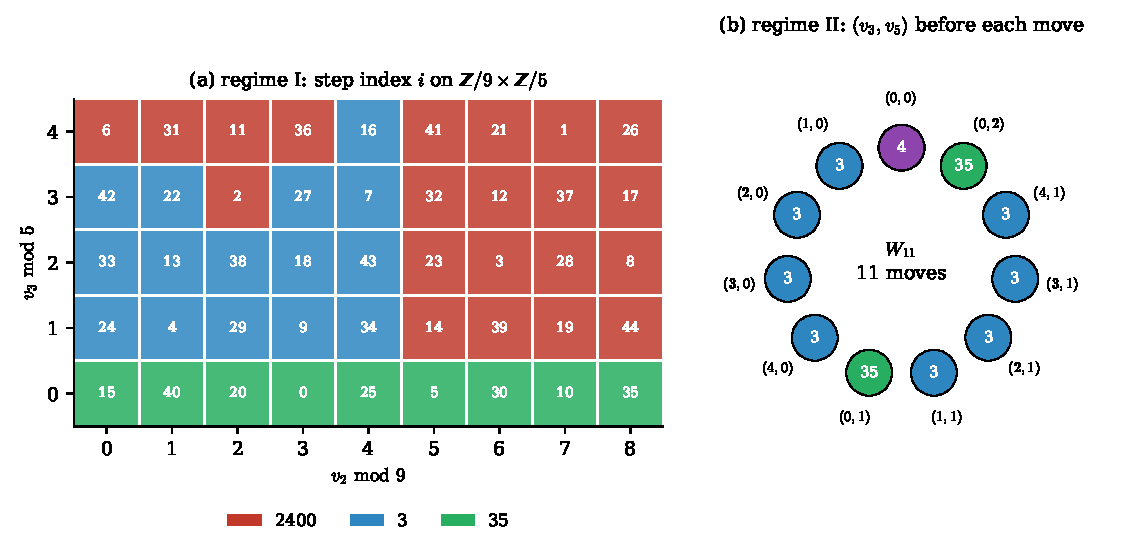
\includegraphics[width=\textwidth]{../figures/fig_registers.pdf}
\caption{The two periodic regimes. (a) Regime I: the $45$ steps of $\Wa$ fill the grid $\mathbb{Z}/9\times\mathbb{Z}/5$ of $(v_2\bmod9,v_3\bmod5)$, numbered by step; colours are the selected move. (b) Regime II: the $11$-cycle of $\Wb$, with the register $(v_3,v_5)$ before each move.}
\label{fig:registers}
\end{figure}

\subsection{Regime II: a register cycle of period 11}

\begin{proposition}[Regime II]\label{prop:reg2}
Consider a stretch of the orbit on which the selected move lies in $\{3,35,4\}$ and: $v_5\le1$ whenever $v_3\ge1$; $v_7\ge1$ before each $35$; $v_2\ge2$ before each $4$. Then:
\begin{enumerate}[label=(\roman*)]
\item the register $(v_3,v_5)$ evolves autonomously by $3:(v_3,v_5)\mapsto(v_3-1,v_5)$ if $v_3\ge1$; $35:(v_3,v_5)\mapsto(v_3+4,v_5-1)$ if $v_3=0,v_5\ge1$; $4:(v_3,v_5)\mapsto(v_3,v_5+2)$ if $v_3=0,v_5=0$;
\item after a finite transient the itinerary is periodic with period $11$: a rotation of $\Wb=(3,3,3,3,35,3,3,3,3,4,35)$, through the register states $(0,2)\to(4,1)\to\dots\to(0,1)\to(4,0)\to\dots\to(0,0)\to(0,2)$;
\item $\Delta(\Wb)=(+38,0,0,-2)$.
\end{enumerate}
\end{proposition}
\begin{proof}
(i) If $v_3\ge1$ then $2400$ is disabled by $v_5\le1$, so the first enabled move is $3$ (priority $2$ of $L_4$). If $v_3=0$ then $2400,3,15,27$ are disabled (each needs a factor $3$); $35$ is enabled iff $v_5\ge1$ (given $v_7\ge1$); otherwise $4$ is the next candidate and is enabled ($v_2\ge2$). (ii) From $(v_3,v_5)$ the moves $3$ reduce $v_3$ to $0$; then each $35$ lowers $v_5$ by one and resets $v_3=4$, followed by four $3$'s; when $v_5=0$ the move $4$ sets $v_5=2$. The cycle through $(0,2)$ is $35,3^4,35,3^4,4$, i.e.\ a rotation of $\Wb$, of length $2\cdot5+1=11$, and every register state flows into it. (iii) The word has eight $3$'s, two $35$'s and one $4$: $\Delta_2=8\cdot4+2\cdot4-2=38$, $\Delta_3=-8+8=0$, $\Delta_5=-2+2=0$, $\Delta_7=-2$.
\end{proof}

\subsection{Regime III: an exactly solvable run}

\begin{proposition}[Regime III]\label{prop:reg3}
If $v_3=v_7=0$ and $v_2=m$, then the orbit continues with $m'=\lfloor m/2\rfloor$ moves $4$ and reaches $(m\bmod 2,\,0,\,v_5+2m',\,0)$; every state before the last has $v_2\ge2$, so none of them lies in $\Sig$.
\end{proposition}
\begin{proof}
$v_3=v_7=0$ disables $2400,3,35,15,27$ (each needs $3$ or $7$), and $4$ is the next entry of $L_4$, enabled while $v_2\ge2$; it adds $(-2,0,+2,0)$ and preserves $v_3=v_7=0$.
\end{proof}

In particular \emph{the final exponent of $5$ in a round is $z'=v_5+(v_2-a')/2$ evaluated at the start of regime III, and $a'=v_2\bmod2$ there.} This part of the return law is exact and needs no computer.

\subsection{The exchange cycle}

\begin{proposition}[Exchange rates and gain]\label{prop:exchange}
The three periods have net vectors
\[
\Delta(\Wa)=(0,0,-49,+151),\qquad \Delta(\Wb)=(+38,0,0,-2),\qquad \Delta(4)=(-2,0,+2,0),
\]
which convert, respectively, $49$ units of $v_5$ into $151$ of $v_7$; $2$ units of $v_7$ into $38$ of $v_2$; and $2$ units of $v_2$ into $2$ of $v_5$. Following one unit of $v_5$ around the cycle $5\to7\to2\to5$ multiplies it by
\[
\frac{151}{49}\cdot\frac{38}{2}\cdot\frac{2}{2}=\frac{151\cdot19}{49}=\frac{2869}{49}\approx58.551 .
\]
\end{proposition}

\noindent The factor $19=38/2$ and the prime $151$ are therefore not fitted numbers; they are $\Delta_2(\Wb)/|\Delta_7(\Wb)|$ and $\Delta_7(\Wa)$. The expansion of the return map, and hence the inequality $z'\ge10z$, is the statement that this cycle gain exceeds $1$ by a wide margin.

\subsection{The balance identity}\label{subsec:balance}

Every certified round program (\S\ref{sec:proof}) has the form: a bounded prefix, $\Wa^{k_1}$, a bounded connector, $\Wb^{k_2}$, a bounded tail, and $4^{k_3}$. Let $P=(P_2,P_3,P_5,P_7)$ be the total net vector of the bounded items (prefix, connector, tail), let $Q_5$ be the net change of $v_5$ over the prefix, and let $e_1$ be the value of $v_5$ immediately after $\Wa^{k_1}$.

\begin{proposition}[Balance identity]\label{prop:balance}
For a round from $(a,0,z,0)$ ending at $(a',0,z',0)$, with the above form:
\begin{enumerate}[label=(\roman*)]
\item $49\,k_1=z+Q_5-e_1$;
\item $2k_2=151\,k_1+P_7$;
\item $2k_3=38\,k_2+(a-a')+P_2$;
\item $z'=z+2820\,k_1+\bigl(P_5+P_2+19P_7+a-a'\bigr)$, hence
\begin{equation}\label{eq:balance}
49z'=2869\,z+\delta,\qquad \delta=2820\,(Q_5-e_1)+49\bigl(P_5+P_2+19P_7+a-a'\bigr).
\end{equation}
\end{enumerate}
\end{proposition}
\begin{proof}
(i) $v_5$ after $\Wa^{k_1}$ is $z+Q_5-49k_1=e_1$. (ii) $v_7=0$ at the end and the net change of $v_7$ is $151k_1+P_7-2k_2$ (the blocks $\Wb$ and $4$ and the bounded items are the only other contributors; $\Delta_7(\Wa)=151$). (iii) The same for $v_2$: $a'=a+P_2+38k_2-2k_3$. (iv) $z'=z+P_5-49k_1+2k_3$ by the net change of $v_5$; substitute (iii) and (ii) to get $2k_3=19(151k_1+P_7)+(a-a')+P_2$, so $z'=z+2820k_1+(P_5+19P_7+P_2+a-a')$; multiply by $49$ and use (i).
\end{proof}

\begin{corollary}[What the identity explains]\label{cor:explains}
For every certified family:
\begin{enumerate}[label=(\alph*)]
\item the slopes of $k_1,k_2,k_3,z'$ in $z$ are $\tfrac1{49},\ \tfrac{151}{98},\ \tfrac{2869}{98},\ \tfrac{2869}{49}$; the lattice of $z$-increments on which all three block counts are integers is $98\Z$, since $\gcd(151,98)=\gcd(2869,98)=1$. This is the origin of the modulus $98$ and of the slopes $2,151,2869$ and $5738=98\cdot2869/49$ in the certificate (with $z=50000+\rho+98t$);
\item integrality of $z'$ forces $\delta\equiv-2869\,z\equiv-27\,r\pmod{49}$ (as $2869\equiv27$);
\item $a'\equiv a+P_2\pmod2$: $a'$ is the parity of $v_2$ at the start of regime III (Proposition~\ref{prop:reg3});
\item $P_7\equiv k_1\pmod 2$: the connector between the two blocks must supply the parity of $v_7$, which is why $z$ is resolved modulo $98$ rather than $49$.
\end{enumerate}
\end{corollary}

All identities of Proposition~\ref{prop:balance} and Corollary~\ref{cor:explains} hold in each of the $196$ certified programs (computed in \texttt{mechanism\_check.py}; data in \texttt{balance\_identity\_196.csv}); in particular $\delta\equiv-27r\pmod{49}$ in all $98$ table entries. The same data show that $Q_5=-1$ for $a=0$ (the round opens with one move $N=5$) and $Q_5=+7$ for $a=1$ (the seven-move prefix of Proposition~\ref{prop:reduction} followed by that move), that $e_1=(r+Q_5)\bmod49\in[0,48]$, and that the two outliers of the correction table, $\delta_{0,25}=4323$ and $\delta_{1,17}=27275$, are exactly the entries with $e_1=24$. As a check, for $(a,\rho)=(0,0)$: $z=50000$, $k_1=1020$, $Q_5=-1$, $e_1=19$ (so $49\cdot1020=50000-1-19$), $P_2=27,\ P_5=-19,\ P_7=52$, $a'=1$, whence $z'=50000+2820\cdot1020+(-19+27+988-1)=2{,}927{,}395$ and $\delta=2820\cdot(-20)+49\cdot995=-7645$, as in Table~\ref{tab:returnmap}.

\subsection{The derivation and the certificate: division of labour}\label{subsec:limits-mech}
Propositions~\ref{prop:reg1}--\ref{prop:exchange} and~\ref{prop:balance} derive, from the vectors $\Delta(N)$ alone: the periods $45$ and $11$ and their net vectors; the exchange rates; the gain $2869/49$; the block slopes; the modulus $98$; the parity rule for $a'$; the congruence $\delta\equiv-27r\pmod{49}$; and the exact closing of the round in regime III. They do not derive the \emph{bounded transients}: the prefix, the connector in which the register of regime I drains $v_5$ from $e_1$ to $\le1$ and hands over to regime II, and the tail in which $v_7$ runs out and regime III begins. These transients fix $Q_5,e_1,P$ and thereby the table of $\delta_{a,r}$. They are finite computations whose legality for \emph{all} $t$ is exactly what the certificate of \S\ref{sec:proof} proves, so the proof of Theorem~\ref{thm:return} uses the computer only for the transients and for the verification that the regimes are entered and left as described.

%% ------------------------------------------------------------------
\section{Proof architecture and the certificate}\label{sec:proof}

\subsection{Parametrisation by families}
Every pair $(a,z)$ with $z\ge50000$ is written uniquely as $z=50000+\rho+98\,t$ with $0\le\rho<98$ and $t\ge0$. This gives $2\times98=196$ \emph{families} $(a,\rho)$, each parametrised by $t\in\N$. By Corollary~\ref{cor:explains}(a), $98$ is the smallest increment of $z$ by which all three block counts change by integers.

\subsection{Round programs}
A \emph{round program} for $(a,\rho)$ is a finite list of items, each either a single move $N\in\mathcal{M}_P$ or a \emph{block} $W^{T(t)}$, a word $W$ of moves repeated $T(t)=c+\kappa t$ times with integers $c,\kappa\ge0$. Running a program from $v^{(0)}(t)=(a,0,50000+\rho+98t,0)$ gives exponent vectors affine in $t$ (and, inside a block, affine in $(t,k)$, $k$ the repetition index): the $j$th move of repetition $k$ of a block starting from $u(t)$ occurs at the state $u(t)+k\Delta(W)+\Delta(w_1\cdots w_{j-1})$.

\subsection{The four obligations}
A program $\mathcal{P}$ is \emph{certified} for the family when the following hold for all $t\ge0$ and (inside blocks) all $0\le k\le T(t)-1$.
\begin{description}[leftmargin=1.2em,itemsep=2pt]
\item[(E)] \emph{Enabled.} The program's move $N$ is admissible at the current state, $v\ge \vp(N)$.
\item[(D)] \emph{Dominant.} Every move of higher priority than $N$ is not admissible: for each such $N'$ some coordinate has $v_i<\vp_i(N')$.
\item[(S)] \emph{No earlier selected return.} No state strictly inside the round satisfies $v_3=v_7=0$, $v_2\in\{0,1\}$, $v_5\ge10z$, where $z=50000+\rho+98t$.
\item[(F)] \emph{Final state.} The state after the last item is $(a',0,z'(t),0)$ with $a'\in\{0,1\}$ constant, $z'(t)$ affine in $t$, and $z'(t)\ge10z(t)$ for all $t\ge0$.
\end{description}

\begin{lemma}[Certified programs give the orbit]\label{lem:cert}
If a program is certified for $(a,\rho)$, then for every $t\ge0$ the orbit of $2^a5^{50000+\rho+98t}$ follows the program move by move, and its selected return is the final state of the program.
\end{lemma}
\begin{proof}
Induct on the steps. By (E) and (D) the selector's choice at each state is the program's move. By (S) no earlier state in the round is a selected return, and by (F) the final state is in $\Sig$ with $z'\ge10z$, hence is the selected return.
\end{proof}

\subsection{Deciding the obligations exactly}
Each of (E), (D), (S) is the statement that a set of integer points is empty. Outside blocks the points are in $t$ alone; inside blocks, in $(t,k)$. A \emph{violation} is a conjunction of linear inequalities $c_tt+c_kk+c_0\ge0$ with integer coefficients (a strict inequality becomes non-strict by integrality; (S) adds the equations $v_3=v_7=0$ and $v_2\in\{0,1\}$ as pairs of inequalities, one value at a time), together with $t\ge0$, $k\ge0$, $T(t)-1-k\ge0$.

\begin{lemma}[Emptiness by vertices]\label{lem:vertex}
Let $\Pi\subset\mathbb{R}^2$ be defined by finitely many inequalities including $t\ge0$ and $k\ge0$. Then $\Pi\ne\emptyset$ iff $\Pi$ has a vertex, i.e.\ a point of $\Pi$ that is the intersection of two non-parallel boundary lines. If $\Pi=\emptyset$ then $\Pi\cap\Z^2=\emptyset$.
\end{lemma}
\begin{proof}
$\Pi$ lies in the quadrant $t,k\ge0$ and contains no line, so it is pointed; a nonempty pointed polyhedron has a vertex (a basic feasible solution), and in $\mathbb{R}^2$ a vertex lies on two independent boundary lines. The last statement is trivial.
\end{proof}

Hence emptiness can be decided by testing the finitely many intersections of pairs of constraint lines in exact rational arithmetic (solver (a)). As a second, independent decision procedure we used Fourier--Motzkin elimination in exact rational arithmetic (solver (b)). In every case treated below the violation set was rationally empty, so no integer fallback was needed.

\begin{example}[One obligation by hand]\label{ex:oblig}
In the program for $(0,0)$ (Appendix~\ref{app:worked}) the block $\Wb^{T}$, $T=77036+151t$, starts at $v_7=154073+302t$ and each repetition consumes $2$ units. The first $35$ of repetition $k$ needs $v_7\ge1$. A violation would satisfy $154073+302t-2k\le0$, $k\le 77035+151t$, $t,k\ge0$. Adding $2\times$ the second inequality to the first gives $154073-154070\le0$, i.e.\ $3\le0$: the set is empty. The slack $3$ is the reason the block can run for exactly $T$ repetitions and not one more: the last repetition leaves $v_7=1$, and the tail's $35$ takes it to $0$.
\end{example}

\subsection{Extracting the programs}
The itinerary shape of each family was extracted by naive simulation at $t=0,\dots,7$ ($1568$ runs), detecting repeated blocks (period $\le64$, at least three repetitions), and fitting block lengths affinely in $t$. This is a \emph{search} and carries no weight in the proof: by Lemma~\ref{lem:cert} a mis-extracted program would fail (E) or (D). Propositions~\ref{prop:reg1} and~\ref{prop:reg2} explain \emph{why} the search finds the words $\Wa,\Wb$ in the long blocks.

\subsection{Result of the certification}\label{subsec:results-cert}
All $196$ programs were certified: $99{,}866$ obligations (E), (D), (S), (F), all empty/satisfied, by both solvers. Every program has the form of \S\ref{subsec:balance}, with $\Wa$ and $\Wb$, up to a cyclic rotation that varies with the family, equal to
\begin{align*}
\Wa&=(2400,2400,3,2400,35,2400,3,3,2400,35,2400,3,2400,3,35,\\
&\qquad 2400,3,2400,3,35,2400,2400,3,2400,35,3,2400,3,2400,35,\\
&\qquad 2400,3,2400,3,35,2400,3,2400,3,35,2400,2400,3,3,35),\\
\Wb&=(3,3,3,3,35,3,3,3,3,4,35),
\end{align*}
and $k_1=c_1+2t$, $k_2=c_2+151t$, $k_3=c_3+2869t$ with family-dependent constants (for $(a,\rho)=(0,0)$: $c_1=1020$, $c_2=77036$, $c_3=1{,}463{,}697$; the constants depend on how repetitions at block boundaries are counted, the slopes do not). A round has $L_0+4620\,t$ moves, $4620=45\cdot2+11\cdot151+2869$, and asymptotically $1.9\%$, $36.0\%$ and $62.1\%$ of its steps lie in the three regimes (Figure~\ref{fig:anatomy}). A complete worked program is in Appendix~\ref{app:worked}, and all $196$ programs are in the supplement (\texttt{programs\_196.csv}).

\begin{figure}[t]
\centering
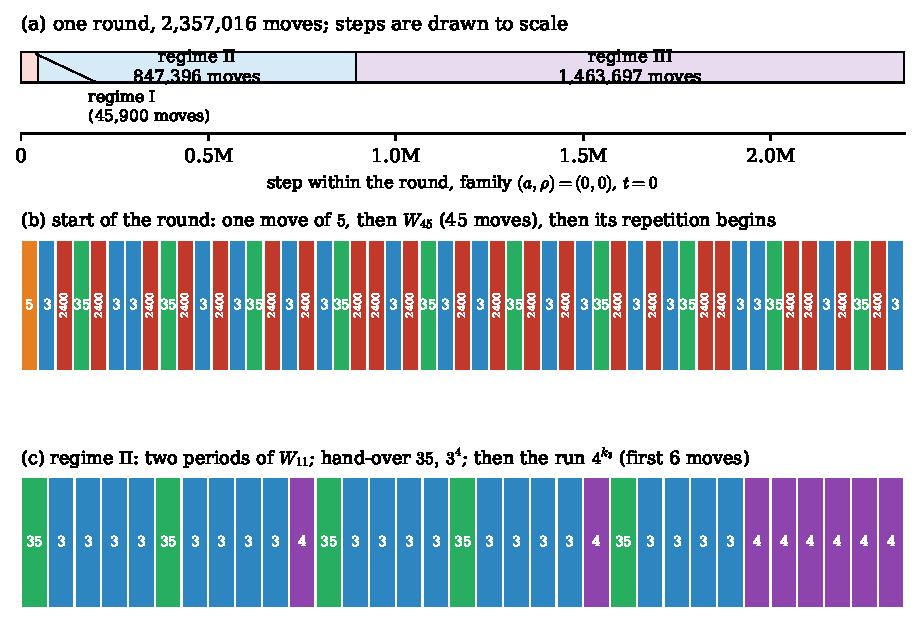
\includegraphics[width=\textwidth]{../figures/fig_anatomy2.pdf}
\caption{Anatomy of one round, family $(a,\rho)=(0,0)$ at $t=0$. (a) The three regimes drawn to scale. (b) The start of the round: the single move $5$, then the $45$ moves of $\Wa$. (c) Two periods of $\Wb$, the hand-over, and the beginning of the run $4^{k_3}$. Colours: $2400$ red, $3$ blue, $35$ green, $4$ purple, $5$ orange.}
\label{fig:anatomy}
\end{figure}

\subsection{Proof of Theorem~\ref{thm:return}}
Existence and the form of $\Ret$ follow from Lemma~\ref{lem:cert} applied to all $196$ families, which cover every $(a,z)$ with $z\ge50000$. The final state of family $(a,\rho)$ is $(a',0,z'(t),0)$ with $z'(t)=\beta+5738\,t$ for a family-dependent $\beta$ and, in all $196$ cases, the same slope $5738$ (which Corollary~\ref{cor:explains}(a) predicts). Since $2869\cdot98=281{,}162=49\cdot5738$,
\[
49\,z'(t)=49\beta+281{,}162\,t=2869\,(z_0+98t)+\delta,\qquad \delta:=49\beta-2869\,z_0,
\]
with $z_0=50000+\rho$ and $\delta$ independent of $t$. This is \eqref{eq:return}. The computed pairs $(a',\delta)$ for $\rho$ and $\rho+49$ coincide in all cases, so they depend on $(a,r)$ only, and the $98$ values are Table~\ref{tab:returnmap}; $\min\delta=-7737$ and $\max\delta=27275$ are attained. Integrality of $z'$ is automatic ($z'$ is an exponent) and agrees with Corollary~\ref{cor:explains}(b). The inequality $z'\ge10z$ is (F); with slope $5738\ge980=10\cdot98$ it holds for all $t$. $\qquad\blacksquare$

\subsection{Proof of Corollary~\ref{cor:orbit}}
The entry step $n_0$ and the state $s_0$ were obtained by direct execution of the selector from $x_0$ (no jumping), checking membership in $\Sig$ at each step; the same run, extended to $3.6\cdot10^9$ steps, found $\Sig$-visits at steps $1{,}039{,}587$; $1{,}039{,}594$ ($(0,1{,}269{,}121)$, the skipped first return, in agreement with Proposition~\ref{prop:reduction}); $60{,}869{,}526$ and $3{,}563{,}973{,}091$. By Theorem~\ref{thm:return} the last two are $\Ret(s_0)$ and $\Ret^2(s_0)$, and the formula predicts both the values and the step numbers. Since $\Ret:\Sig\to\Sig$ is total and $z_{j+1}\ge10z_j$, the orbit visits all $s_j$ in order. The round length $L_0+4620t$ is the sum of the block lengths of the certified program, whose slope is $4620$. The entry is a verified computation, not a symbolic reachability proof. $\qquad\blacksquare$

\subsection{Proof of Theorem~\ref{thm:aper}}\label{sec:aper}
For each family, the last item of the certified program is $4^{k_3}$ with $k_3=c_3+2869t$, $c_3\ge1{,}463{,}697$, and the first move is $N=2$ or $N=5$ (verified over the $196$ programs; for $a=1$ the first move is $2$, for $a=0$ it is $5$). In the chain of rounds the last move of one round and the first move of the next are consecutive in the itinerary. Since $z_j\ge 10^jz_0$, $t_j\to\infty$, so the itinerary contains runs $4^{\ell_j}$, $\ell_j\ge 2869\,t_j\to\infty$, each immediately followed by a move $\ne4$.

Suppose the itinerary were eventually periodic with period $q$ from index $n_*$. Choose $j$ so large that the run $4^{\ell_j}$ lies after $n_*$ and $\ell_j\ge q$. Within the periodic tail any $q$ consecutive symbols contain a full period, so a window of $q$ equal symbols forces the period word to be $4^q$; then every later symbol is $4$, contradicting the move $\ne 4$ that immediately follows the run. $\qquad\blacksquare$

\begin{remark}[A second route]
The blocks $\Wa^{k_1}$ and $\Wb^{k_2}$ also have unbounded lengths. Suppose the itinerary had eventual period $q$, with period word $w$. A stretch of the tail inside a long power of the primitive word $\Wa$ has periods $45$ and $q$; by the Fine--Wilf theorem \cite{finewilf} (length $\ge 45+q-\gcd(45,q)$) it has period $\gcd(45,q)$, which by primitivity forces $45\mid q$, and then $w$ is a conjugate of $\Wa^{q/45}$. The same argument with $\Wb$ makes $w$ a conjugate of $\Wb^{q/11}$. The primitive root of a word is unique up to conjugacy, so $\Wa$ and $\Wb$ would be conjugate, which is impossible since their lengths differ. This second proof is independent of the run of $4$'s; both rest on the same certified block structure.
\end{remark}

%% ------------------------------------------------------------------
\section{Independent verification}\label{sec:audit}

The result was first certified in a frozen release \cite{adj4-frozen} and then re-derived in a separate package \cite{adj4-audit} written from the specification (Definitions~\ref{def:moves}--\ref{def:section}) and the stored priority list only, without importing code from the original. The audit consisted of:
\begin{itemize}
\item an independent implementation of the selector and move set (the $22$ moves recomputed; the vector update checked against literal integer arithmetic on $20{,}000$ random states; a big-integer orbit matched the vector orbit for $3000$ steps);
\item the symbolic certification of all $196$ families by a new implementation with two independent emptiness solvers, agreeing on all $99{,}866$ obligations and on $300{,}000$ random instances;
\item cross-validation of the fitted programs by naive simulation at $48$ sampled large parameters (up to $t=20{,}000$, with single rounds of up to about $9.5\cdot10^7$ steps), with no mismatch in itinerary shape, $z'$, $a'$ or step count;
\item negative controls, all rejected: lengthening blocks by one repetition ($588/588$), shortening interior blocks ($392/392$), shortening the final run ($196/196$, caught by (F)), and swapping two priorities ($196/196$);
\item direct execution to $3.6\cdot10^9$ steps and comparison of the visits with the prediction of Theorem~\ref{thm:return} (Corollary~\ref{cor:orbit});
\item comparison with the original table: $a'$, the intercept and slope of $z'$ and $\delta$ agree in $196/196$ families. Block-repetition counts differ by a constant $3$ in each block because the two tokenisers count the initial repetitions of a block differently; slopes, itineraries and endpoints are identical.
\end{itemize}

\paragraph{Checks added in the present version.} These are computations on the audit's stored outputs, not re-runs of the certificate (the certificate itself was \emph{not} re-run for this version; the inherited files are listed with SHA-256 hashes in the supplement): (i) the balance identity of Proposition~\ref{prop:balance} and Corollary~\ref{cor:explains} in all $196$ programs (\texttt{mechanism\_check.py}); (ii) the register-cycle statements of Propositions~\ref{prop:reg1}--\ref{prop:reg2}: the automaton $F$ on $(v_2,v_3)\in[0,399]\times[0,11]$ has a single cycle, of length $45$, with the stated counts and net vector, the closed form reproduces $\Wa$ exactly, and the $11$-cycle of $\Wb$ (\texttt{register\_cycles.py}); (iii) the seven-move lemma and the $49$-residue table identity of Proposition~\ref{prop:reduction} (\texttt{reduction\_check.py}); (iv) the affine step law $L_0+4620t$ for all $196$ families at $t=0,\dots,7$ (\texttt{orbit\_predictions.py}).

\paragraph{Independence of the verification.} The audit is independent in implementation and method: it was written from the original specification by separate implementations within the research collective. The package includes reproduction steps for any reader who wishes to examine the certificate.

%% ------------------------------------------------------------------
\section{Mathematical correspondences and methods}\label{sec:relation}

\subsection{Representation of the fixed-priority selector}\label{subsec:fractran}
A program in Conway's FRACTRAN \cite{conway87,conway72} is an ordered list of rational multipliers $f_1,\dots,f_n$; from an integer $x$ one multiplies by the first $f_i$ for which $f_ix\in\Z$.

\begin{proposition}[Ordered rational-multiplier form]\label{prop:fractran}
For a fixed priority list $L=(N_1,\dots,N_n)$, the autonomous selector of Definition~\ref{def:selector} and its orbit $x_{k+1}=x_k\nest\sigma_L(x_k)$ coincide exactly with the FRACTRAN program with the ordered fractions $(N_1+1)^2/N_1,\dots,(N_n+1)^2/N_n$. In particular the four-prime system is such a program with $22$ fractions, and the itinerary is the sequence of fractions applied.
\end{proposition}
\begin{proof}
The fraction $(N+1)^2/N$ is in lowest terms. For an integer $x$, $x(N+1)^2/N\in\Z$ iff $N\mid x$ (Lemma~\ref{lem:anchor}). Hence the first fraction that produces an integer is the first $N_i\mid x$.
\end{proof}
The proposition concerns the fixed-priority selector of \S\ref{sec:selection} and is stated for that rule alone. The results of this paper, the expanding return theorem on the section $\Sig$ (Theorem~\ref{thm:return}) and the itinerary of the designated orbit (Theorem~\ref{thm:aper}), are statements about the dynamics of this selector which the proposition does not address.

\subsection{Mathematical methods}\label{subsec:methods}
The proofs combine five methods. \emph{Prime valuations:} each move $N$ translates the exponent vector of the state by a fixed vector $\Delta(N)$ above a threshold $\vp(N)$, so that the dynamics is read in exponent coordinates (\S\ref{sec:grammar}). \emph{Finite-state rotations:} the top three moves act as a rotation on $\mathbb{Z}/9\times\mathbb{Z}/5$ with period $45$, and the remaining register evolves on a cycle of period $11$ (\S\ref{sec:mechanism}). \emph{Exponent-transfer identities:} the exchange cycle and the balance identity give the gain $2869/49$, the block slopes and the congruence for $\delta$ directly from the vectors $\Delta(N)$. \emph{Return maps:} the selected return on $\Sig$ reduces an unbounded orbit to an explicit expanding map with a periodic correction (\S\ref{sec:results}). \emph{Exact certification:} the finite families of bounded transients are decided by exact emptiness of rational polyhedra, excluding integer violations, with independent re-implementation (\S\ref{sec:proof}, \S\ref{sec:audit}). The word-combinatorial second proof of Theorem~\ref{thm:aper} uses the Fine--Wilf theorem \cite{finewilf}, and the move set consists of the pairs $N,N+1$ that are both $\{2,3,5,7\}$-smooth \cite{stormer,lehmer,oeis}.
We examined the FRACTRAN and generalized-Collatz literature \cite{kurtzsimon,endrullis,monks,goncalves,lagarias}, the BusyBeaverWiki description of FRACTRAN programs \cite{bbwiki} and the literature on exact renormalisation for piecewise-affine maps \cite{schwartz,akiyama} in preparing this paper, and claim only the theorems proved here.

%% ------------------------------------------------------------------
\section{Mathematical significance and consequences}\label{sec:signif}

\paragraph{The central result.} On the section $\Sig$ the selected return is exactly
\[
\mathcal R(a,z)=\Bigl(a',\ \frac{2869\,z+\delta_{a,r}}{49}\Bigr),\qquad r=z\bmod49,
\]
and its structure is explained by the exchange cycle
\[
v_5\longrightarrow v_7\longrightarrow v_2\longrightarrow v_5,\qquad \frac{2869}{49}=\frac{151}{49}\cdot19\cdot1 .
\]
Three locally periodic arithmetic regimes combine into an expanding generative process with a certified non-eventually-periodic selection itinerary.


\paragraph{Autonomous arithmetic organisation.} A purely local, stationary, input-free selection rule over a finite list of generative acts, with no counter, clock or external instruction, organises its own long-range behaviour. The state chooses the next act through divisibility alone, and the resulting dynamics on the section $\Sig$ is governed by an exact renormalisation: the explicit expanding map $z\mapsto(2869z+\delta_{a,r})/49$ with a finite correction table.

\paragraph{Periodic subsystems, aperiodic itinerary.} Each round is assembled from subsystems that are themselves exactly periodic: a rotation on $\mathbb{Z}/9\times\mathbb{Z}/5$ among the top three moves with period $45$, and a register cycle with period $11$. Their blocks of unbounded length, arranged by the exchange cycle, produce an itinerary that is not eventually periodic (Theorem~\ref{thm:aper}); the Fine--Wilf argument of its second proof shows that the two periodic blocks cannot be absorbed into any single period.

\paragraph{Exponent-transfer amplification.} The exchange cycle $5\to7\to2\to5$ moves the exponent of $5$ into $7$, then $2$, then $5$ at the rates $151/49$, $19$ and $1$. The gain $2869/49=\frac{151}{49}\cdot19\cdot1$ is therefore a product of exchange rates read from the vectors $\Delta(N)$; so are the block slopes, the modulus $98$, the parity rule for $a'$ and the congruence $\delta\equiv-27r\pmod{49}$, which trace to $9=5+4$ and $5=1+4$ in regime I (\S\ref{sec:mechanism}).

\paragraph{Exact return predictability.} The selected return is determined exactly, not statistically: round lengths are $L_0(a,\rho)+4620\,t$, each round is scaled by about $2869/49$, and the three regimes occupy asymptotically fixed proportions of approximately $1.9\%$, $36.0\%$ and $62.1\%$ (in each round these proportions are perturbed only by the family-dependent intercepts). The itinerary is hierarchical and asymptotically self-similar under $\Ret$.

\paragraph{Local admissibility and global dynamics.} The only local datum is which nests anchor the current integer. The three regimes, the periods and the expansion factor all follow from this datum together with the priority order, which shows how a purely local admissibility rule fixes a global exponent dynamics.

\paragraph{What is established, and how.} The expanding return theorem applies throughout the section $\Sig$, while the designated initial orbit provides an explicitly computed entry into that section (Theorem~\ref{thm:return} and Corollary~\ref{cor:orbit}). The expansion mechanism is derived from the arithmetic transition vectors, and the finite connecting transients are established by exact computational certification across all $196$ parameter families, with independent re-implementation (\S\ref{sec:proof}--\ref{sec:audit}).

\paragraph{Further mathematical directions.} (a) A structural derivation of the transient maps, that is, of the table $\delta_{a,r}$ as a function of the residual $e_1$, whose dependence on $e_1$ has slope $-2820$, a $5$-periodic pattern and one exceptional residual $e_1=24$. (b) A symbolic account of the entry into $\Sig$. (c) The behaviour of other priority orders on the same move set, and of other orbits of $L_4$. (d) Whether the exchange-cycle mechanism, a rotation on $\mathbb{Z}/m\times\mathbb{Z}/n$ with $m,n$ the sums of the two possible changes of a coordinate, occurs for other prime sets.

\section{Data and code availability}
The frozen certificate release is \texttt{UNNS\_GUP\_ADJ4\_v001} (SHA-256 \texttt{\seqsplit{29afeadc54dbf04a424e6f9fb16c36230cd7bd5ae71d191107e7c580932551c7}}). The audit package \texttt{UNNS\_GUP\_ADJ4\_AUDIT\_v001} (SHA-256 \texttt{\seqsplit{e2592db3358b2b1c960489eabf8c6a60b07616e5bf4b65e73df3114dd0e8b7db}}) contains the independent source code, all certificate outputs, the large-parameter cross-validation, negative controls and a one-command reproducer. Neither was modified, and neither is part of the GitHub source collection described next. The arithmetic grammar underlying the construction (the transition $x\mapsto x(N+1)^2/N$, the arithmetic graph, the prime-valuation reduction and the finite-control selector background) is documented in the research source collection \cite{ad-collection}, pinned to commit \texttt{22d8c2e23f49fb98a5b04c6b7efe9ba0a3703808}; the relevant releases there are \texttt{UNNS\_U4\_GEN\_v001} \cite{u4gen} (prime-valuation generation and the selector $\textsf{MAXPP}$) and \texttt{UNNS\_U2\_001\_v001} \cite{u2001} (finite-control selectors and arithmetic routes). These sources support the arithmetic grammar only; the ADJ4 priority order, the expanding return theorem and the certificate are recorded solely in the two packages named above. The present package \texttt{UNNS\_AUT\_APER\_v009} contains the manuscript sources, figures, the scripts that produce every figure and every check of \S\ref{sec:audit}, the list of the $196$ programs, the balance-identity data, and copies of the inherited audit files used (with hashes; these were not re-run).

%% ------------------------------------------------------------------
\begin{thebibliography}{99}\small
\bibitem{unns-intro} UNNS Research Division, \emph{Introduction to the UNNS Substrate: Nested Generation, Route, Boundary, and Admissibility}, 2026; \url{https://unns.tech}.
\bibitem{adj4-frozen} UNNS Research Collective, \emph{UNNS\_GUP\_ADJ4\_v001} (frozen certificate release), 2026.
\bibitem{adj4-audit} UNNS Research Collective, \emph{UNNS\_GUP\_ADJ4\_AUDIT\_v001} (independent certificate audit), November 2026.
\bibitem{ad-collection} UNNS Research Collective, \emph{UNNS Arithmetic Dynamics: Arithmetic Geometry, Generative Routes, Graph Structure, and Symbolic Dynamics in the UNNS Substrate}, research source collection, repository \texttt{ukbbi/UNNS}, directory \texttt{projects/UNNS\_ARITHMETIC\_DYNAMICS}, commit \texttt{22d8c2e23f49fb98a5b04c6b7efe9ba0a3703808}; \url{https://github.com/ukbbi/UNNS/tree/22d8c2e23f49fb98a5b04c6b7efe9ba0a3703808/projects/UNNS_ARITHMETIC_DYNAMICS}.
\bibitem{u4gen} UNNS Research Collective, \emph{UNNS\_U4\_GEN\_v001} (Intrinsic branching and autonomous generative dynamics), release archive SHA-256 \texttt{\seqsplit{042eb5b09b4d231283c9c7d9d40e29a8789625f4b073e724000d49f6d49e18df}}; source record: \url{https://github.com/ukbbi/UNNS/tree/22d8c2e23f49fb98a5b04c6b7efe9ba0a3703808/projects/UNNS_ARITHMETIC_DYNAMICS/04_symbolic_dynamics/UNNS_U4_GEN_v001}.
\bibitem{u2001} UNNS Research Collective, \emph{UNNS\_U2\_001\_v001} (Intrinsic generative selectors), release archive SHA-256 \texttt{\seqsplit{561a9558f713faa2905be18f2a6afc2d3aac6de955c58e73cace7051e057ca21}}; source record: \url{https://github.com/ukbbi/UNNS/tree/22d8c2e23f49fb98a5b04c6b7efe9ba0a3703808/projects/UNNS_ARITHMETIC_DYNAMICS/02_routes_selectors/UNNS_U2_001_v001}.
\bibitem{conway72} J.\,H. Conway, Unpredictable iterations, \emph{Proc.\ 1972 Number Theory Conf.}, Univ.\ Colorado, Boulder, 49--52.
\bibitem{conway87} J.\,H. Conway, FRACTRAN: a simple universal programming language for arithmetic, in T.\,M. Cover and B. Gopinath (eds.), \emph{Open Problems in Communication and Computation}, Springer, 1987, 4--26.
\bibitem{kurtzsimon} S.\,A. Kurtz and J. Simon, The undecidability of the generalized Collatz problem, in \emph{TAMC 2007}, LNCS 4484, Springer, 2007, 542--553.
\bibitem{endrullis} J. Endrullis, C. Grabmayer and D. Hendriks, Complexity of Fractran and productivity, arXiv:0903.4366, 2009.
\bibitem{monks} K.\,G. Monks, $3x+1$ minus the $+$, \emph{Discrete Math.\ Theor.\ Comput.\ Sci.} \textbf{5} (2002), 47--54.
\bibitem{goncalves} F. Gon\c{c}alves, R. Greenfeld and J. Madrid, Generalized Collatz maps with almost bounded orbits, arXiv:2111.06170, 2021.
\bibitem{lagarias} J.\,C. Lagarias, The $3x+1$ problem: an overview, in \emph{The Ultimate Challenge: the $3x+1$ Problem}, AMS, 2010, 3--29.
\bibitem{stormer} C. St{\o}rmer, Quelques th\'eor\`emes sur l'\'equation de Pell $x^2-Dy^2=\pm1$ et leurs applications, \emph{Skr.\ Vid.-Selsk.\ Christiania}, 1897.
\bibitem{lehmer} D.\,H. Lehmer, On a problem of St{\o}rmer, \emph{Illinois J.\ Math.} \textbf{8} (1964), 57--79.
\bibitem{oeis} OEIS Foundation, sequences A002071 and A117581 (consecutive pairs of smooth numbers); \url{https://oeis.org}.
\bibitem{schwartz} R.\,E. Schwartz, Unbounded orbits for outer billiards I, \emph{J.\ Mod.\ Dyn.} \textbf{1} (2007), 371--424; arXiv:math/0702073.
\bibitem{akiyama} S. Akiyama, H. Brunotte, A. Peth\H{o} and W. Steiner, Periodicity of certain piecewise affine planar maps, \emph{Tsukuba J.\ Math.} \textbf{32} (2008), 197--251.
\bibitem{finewilf} N.\,J. Fine and H.\,S. Wilf, Uniqueness theorems for periodic functions, \emph{Proc.\ Amer.\ Math.\ Soc.} \textbf{16} (1965), 109--114.
\bibitem{bbwiki} BusyBeaverWiki, \emph{Fractran} (vector representation of FRACTRAN programs and deciders), \url{https://wiki.bbchallenge.org/wiki/Fractran}, accessed 11 November 2026.
\end{thebibliography}

\appendix
\section{The $22$ moves}
\begin{table}[h]
\centering\small
\begin{tabular}{@{}rrllcr@{}}
\toprule
Priority & $N$ & $N$ & $N+1$ & $\Delta(N)=(\Delta_2,\Delta_3,\Delta_5,\Delta_7)$ & $(N+1)^2/N$\\
\midrule
1 & 2400 & $2^{5}\cdot 3\cdot 5^{2}$ & $7^{4}$ & $(-5,-1,-2,+8)$ & 2402 \\
2 & 3 & $3$ & $2^{2}$ & $(+4,-1,+0,+0)$ & 5.333 \\
3 & 35 & $5\cdot 7$ & $2^{2}\cdot 3^{2}$ & $(+4,+4,-1,-1)$ & 37.03 \\
4 & 15 & $3\cdot 5$ & $2^{4}$ & $(+8,-1,-1,+0)$ & 17.07 \\
5 & 27 & $3^{3}$ & $2^{2}\cdot 7$ & $(+4,-3,+0,+2)$ & 29.04 \\
6 & 4 & $2^{2}$ & $5$ & $(-2,+0,+2,+0)$ & 6.25 \\
7 & 14 & $2\cdot 7$ & $3\cdot 5$ & $(-1,+2,+2,-1)$ & 16.07 \\
8 & 2 & $2$ & $3$ & $(-1,+2,+0,+0)$ & 4.5 \\
9 & 5 & $5$ & $2\cdot 3$ & $(+2,+2,-1,+0)$ & 7.2 \\
10 & 48 & $2^{4}\cdot 3$ & $7^{2}$ & $(-4,-1,+0,+4)$ & 50.02 \\
11 & 4374 & $2\cdot 3^{7}$ & $5^{4}\cdot 7$ & $(-1,-7,+8,+2)$ & 4376 \\
12 & 80 & $2^{4}\cdot 5$ & $3^{4}$ & $(-4,+8,-1,+0)$ & 82.01 \\
13 & 63 & $3^{2}\cdot 7$ & $2^{6}$ & $(+12,-2,+0,-1)$ & 65.02 \\
14 & 125 & $5^{3}$ & $2\cdot 3^{2}\cdot 7$ & $(+2,+4,-3,+2)$ & 127 \\
15 & 224 & $2^{5}\cdot 7$ & $3^{2}\cdot 5^{2}$ & $(-5,+4,+4,-1)$ & 226 \\
16 & 6 & $2\cdot 3$ & $7$ & $(-1,-1,+0,+2)$ & 8.167 \\
17 & 24 & $2^{3}\cdot 3$ & $5^{2}$ & $(-3,-1,+4,+0)$ & 26.04 \\
18 & 49 & $7^{2}$ & $2\cdot 5^{2}$ & $(+2,+0,+4,-2)$ & 51.02 \\
19 & 9 & $3^{2}$ & $2\cdot 5$ & $(+2,-2,+2,+0)$ & 11.11 \\
20 & 8 & $2^{3}$ & $3^{2}$ & $(-3,+4,+0,+0)$ & 10.12 \\
21 & 20 & $2^{2}\cdot 5$ & $3\cdot 7$ & $(-2,+2,-1,+2)$ & 22.05 \\
22 & 7 & $7$ & $2^{3}$ & $(+6,+0,+0,-1)$ & 9.143 \\
\bottomrule
\end{tabular}
\caption{The move set $\mathcal{M}_P$ in priority order (the list $L_4$). Multipliers are rounded to four significant digits.}
\label{tab:moves}
\end{table}

\section{The correction table of the return map}
The table lists both $a=0$ and $a=1$. By Proposition~\ref{prop:reduction} the $a=1$ half is determined by the $a=0$ half: $a'_{1,r}=a'_{0,r+8}$ and $\delta_{1,r}=\delta_{0,r+8}+22{,}952$ (indices mod $49$).
\begin{longtable}{@{}rrrrr@{}}
\caption{Values of $(a',\delta_{a,r})$ in \eqref{eq:return}; $r=z \bmod 49$. Both $a=0$ and $a=1$ are listed. There are $98$ entries; $\min\delta=-7737$, $\max\delta=27275$.}\label{tab:returnmap}\\
\toprule
$r$ & $a'$ ($a=0$) & $\delta_{0,r}$ & $a'$ ($a=1$) & $\delta_{1,r}$\\
\midrule
\endfirsthead
\toprule
$r$ & $a'$ ($a=0$) & $\delta_{0,r}$ & $a'$ ($a=1$) & $\delta_{1,r}$\\
\midrule
\endhead
0 & 1 & $-6\,517$ & 1 & $21\,511$ \\
1 & 0 & $-2\,379$ & 1 & $18\,691$ \\
2 & 0 & $-5\,199$ & 1 & $15\,871$ \\
3 & 0 & $-1\,600$ & 0 & $20\,009$ \\
4 & 1 & $-3\,979$ & 0 & $17\,189$ \\
5 & 1 & $-6\,799$ & 1 & $21\,229$ \\
6 & 0 & $-2\,661$ & 1 & $18\,409$ \\
7 & 0 & $-5\,481$ & 1 & $15\,589$ \\
8 & 1 & $-1\,441$ & 0 & $19\,727$ \\
9 & 1 & $-4\,261$ & 0 & $16\,907$ \\
10 & 1 & $-7\,081$ & 1 & $20\,947$ \\
11 & 0 & $-2\,943$ & 1 & $18\,127$ \\
12 & 0 & $-5\,763$ & 1 & $15\,307$ \\
13 & 1 & $-1\,723$ & 0 & $19\,445$ \\
14 & 1 & $-4\,543$ & 0 & $16\,625$ \\
15 & 1 & $-7\,363$ & 1 & $20\,665$ \\
16 & 0 & $-3\,225$ & 1 & $17\,845$ \\
17 & 0 & $-6\,045$ & 1 & $27\,275$ \\
18 & 1 & $-2\,005$ & 0 & $19\,163$ \\
19 & 1 & $-4\,825$ & 0 & $16\,343$ \\
20 & 1 & $-7\,645$ & 1 & $20\,383$ \\
21 & 0 & $-3\,507$ & 1 & $17\,563$ \\
22 & 0 & $-6\,327$ & 0 & $21\,701$ \\
23 & 1 & $-2\,287$ & 0 & $18\,881$ \\
24 & 1 & $-5\,107$ & 0 & $16\,061$ \\
25 & 1 & $4\,323$ & 1 & $20\,101$ \\
26 & 0 & $-3\,789$ & 1 & $17\,281$ \\
27 & 0 & $-6\,609$ & 0 & $21\,419$ \\
28 & 1 & $-2\,569$ & 0 & $18\,599$ \\
29 & 1 & $-5\,389$ & 0 & $15\,779$ \\
30 & 0 & $-1\,251$ & 1 & $19\,819$ \\
31 & 0 & $-4\,071$ & 1 & $16\,999$ \\
32 & 0 & $-6\,891$ & 0 & $21\,137$ \\
33 & 1 & $-2\,851$ & 0 & $18\,317$ \\
34 & 1 & $-5\,671$ & 0 & $15\,497$ \\
35 & 0 & $-1\,533$ & 1 & $19\,537$ \\
36 & 0 & $-4\,353$ & 1 & $16\,717$ \\
37 & 0 & $-7\,173$ & 0 & $20\,855$ \\
38 & 1 & $-3\,133$ & 0 & $18\,035$ \\
39 & 1 & $-5\,953$ & 0 & $15\,215$ \\
40 & 0 & $-1\,815$ & 1 & $19\,255$ \\
41 & 0 & $-4\,635$ & 1 & $16\,435$ \\
42 & 0 & $-7\,455$ & 0 & $20\,573$ \\
43 & 1 & $-3\,415$ & 0 & $17\,753$ \\
44 & 1 & $-6\,235$ & 0 & $21\,352$ \\
45 & 0 & $-2\,097$ & 1 & $18\,973$ \\
46 & 0 & $-4\,917$ & 1 & $16\,153$ \\
47 & 0 & $-7\,737$ & 0 & $20\,291$ \\
48 & 1 & $-3\,697$ & 0 & $17\,471$ \\
\bottomrule
\end{longtable}


\section{A complete worked program}\label{app:worked}
Table~\ref{tab:worked} gives the certified round program of the family $(a,\rho)=(0,0)$, i.e.\ $z=50000+98t$, as produced by the certificate (the state before each item is affine in $t$; inside a block it is further shifted by $k\,\Delta(W)$, $0\le k<T(t)$). The seventeen connector moves are
\[\begin{gathered}3,2400,35,2400,3,3,2400,35,2400,\\3,2400,3,35,2400,3,2400,3.\end{gathered}\]
 The last column counts the obligations (E), (D), (S) of this item; their sum is $465$, the number reported by the certificate for this family. Obligations are generated at each position $m$ of an item, in number $4$ (E, one per coordinate) $+\,\mathrm{idx}(m)$ (D, one per higher-priority move) $+\,1$ (S), where $\mathrm{idx}(m)$ is the $0$-based priority index of the move. The final state is $(1,0,2{,}927{,}395+5738t,0)$ and $z'(t)\ge10z(t)$ holds for all $t\ge0$ since $2{,}927{,}395\ge500{,}000$ and $5738\ge980$. Example~\ref{ex:oblig} works one obligation through.

\begin{table}[h]
\centering\small
\footnotesize\setlength{\tabcolsep}{3pt}
\begin{tabular}{@{}rllrrrrr@{}}
\toprule
\# & item & repetitions & $v_2$ & $v_3$ & $v_5$ & $v_7$ & obligations\\
\midrule
1 & $5$ & 1 & $0$ & $0$ & $50\,000+98t$ & $0$ & 13 \\
2 & $W_{45}$ & $1\,020+2t$ & $2$ & $2$ & $49\,999+98t$ & $0$ & 259 \\
3 & connector (17 moves) & 1 & $2$ & $2$ & $19$ & $154\,020+302t$ & 98 \\
4 & $W_{11}$ & $77\,036+151t$ & $7$ & $0$ & $2$ & $154\,073+302t$ & 72 \\
5 & $35$ & 1 & $2\,927\,375+5738t$ & $0$ & $2$ & $1$ & 7 \\
6 & $3$ & $4$ & $2\,927\,379+5738t$ & $4$ & $1$ & $0$ & 6 \\
7 & $4$ & $1\,463\,697+2869t$ & $2\,927\,395+5738t$ & $0$ & $1$ & $0$ & 10 \\
\bottomrule
\end{tabular}
\caption{The certified round program for $(a,\rho)=(0,0)$. Columns $v_2,\dots,v_7$ give the state \emph{before} the item (for a block, before its first repetition).}
\label{tab:worked}
\end{table}

\section{Reproducing the checks}\label{app:repro}
The supplement contains, in \texttt{code/}: \texttt{mechanism\_check.py} (balance identity, $196$ families), \texttt{register\_cycles.py} (regimes I--II), \texttt{reduction\_check.py} (Proposition~\ref{prop:reduction}), \texttt{orbit\_predictions.py} (Table~\ref{tab:returns} and the step law), \texttt{program\_table.py}, \texttt{worked\_table.py} and \texttt{figures.py}; \texttt{run\_all.sh} runs them in order in about one minute. They read only the inherited audit files in \texttt{inherited/}, whose SHA-256 hashes are recorded in \texttt{INHERITED\_SHA256SUMS.txt}. The certificate itself is not re-run by these scripts; its one-command reproducer is part of the audit package.


\end{document}
